\chapter{Introduction}\label{chap:intro}

\section{Filebench}
\paragraph{}
Filebench is a framework for simulating different file systems workloads. Such simulation is
helpful to identify performance weaknesses and bottlenecks in file systems. 
Filebench interface relies on an interpreter that reads workload Definition language scenarios in \verb+f+ scripts files.
The model language is expressive which allows Filebench to run so complicated
testing workloads. Filebench at the same time hides the complexity of running multi threaded systems and synchronizing them. Moreover, it offers
an integrated system to measure the latency and throughput for each operation\cite{web:fb-main}.

\paragraph{}
Nowadays, complex applications such as relational databases have sophisticated relations in the system. Setting up each 
application in environment that already has other applications can complicate the benchmarking 
and make it hard to evaluate the results. Filebench gives the power to simulate an application from the
perspective of the filesystem isolating any other interactions that the application can have with other
components of the system.


\section{SDFS}

\paragraph{}
Deduplication becomes more important because of the new features 
that nowadays file systems are offerings as backups and snapshots.
Such features keeps a lot of redundant data on the storage medium.
Cloud computing is forcing more challenges on file systems running
on servers in terms of scalability and storage footprint. Many
of the virtualization environments are keeping copies of the operating systems
images running on the system. Most of those images are similar to large extent
that deduplication can be so useful\cite{usenix}.

\paragraph{}
SDFS is a open source project to implement a file system with deduplication support. Deduplication is a technique
used to save disk space by keeping track of redundant data and save only one copy of that data. Deduplication differs
from compression that the scope of redundancy that has to be avoided is across the file system and on file or at
 least chunks of the file basis. On the other hand compression tries to reduce the size of a file by looking at its byte stream.

\paragraph{}
SDFS offers two mechanism to achieve deduplication: inline and batch mechanisms. The inline mechanism stores chunks of the files and
take a finger print of each chunk by calculating the hash function of the data and then write it directly to storage medium. In case
a similar chunk or file has to be written again, SDFS does not write it instead just references to the existing chunk on the disk.
The batch mode applies a post-process deduplication. The data is stored directly to the disk then the file system perdiodically checks 
for any chance of duplicated chunks.



\paragraph{}
SDFS is implemented as a userspace file system and it is written in JAVA. This gives flexibility to use SDFS without updating the system.
Beside that implementing it in JAVA makes it easier to support multiple operating systems.
\begin{figure}
\label{fig:fuse}
\begin{center}
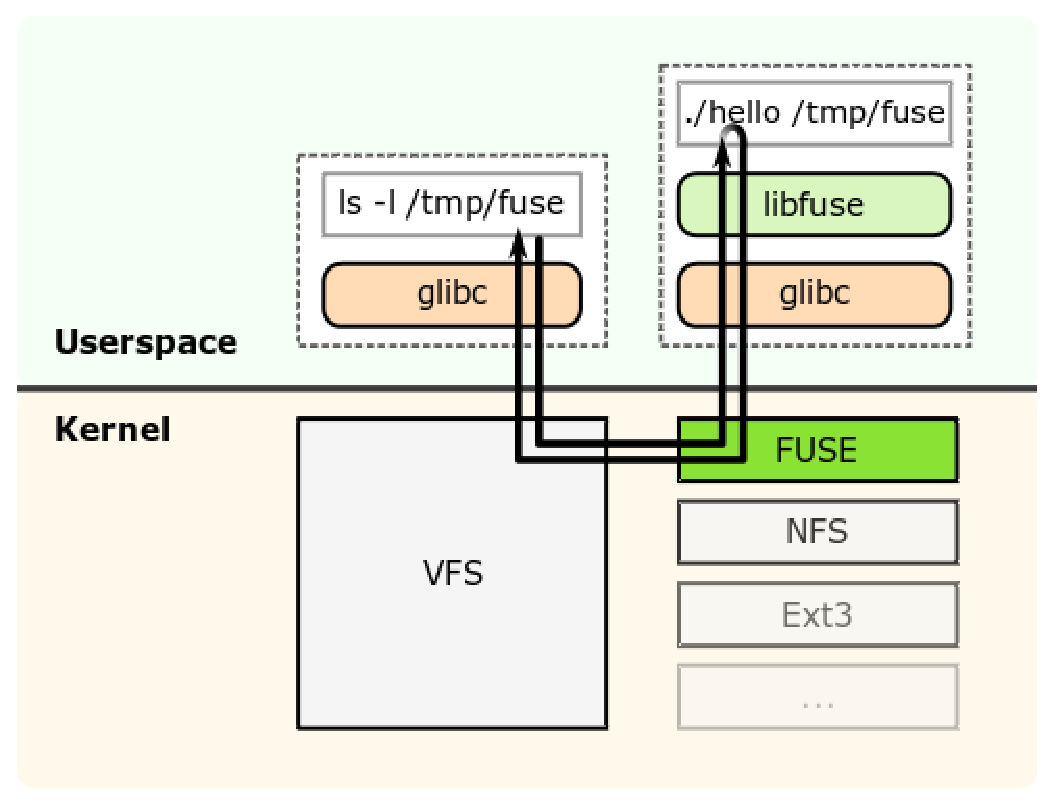
\includegraphics[scale=.55]{FUSE.eps}
\caption{Userspace file system architecture in linux\cite{web:wiki-fuse}}
\end{center}
\end{figure}

\paragraph{}
From figure \ref{fig:fuse}, it is clear the userspace file systems has a lot of similarity of stackable file systems. They allow the developer
to add functionality to an existing file system without changing it. Moreover, they give the flexibility to make such improvements without 
updating the operating system. Userspace performance may suffer due to the extra communication overhead and context switching between kernel and userspace.
However, it has a security advantage by reducing the size of code base runs in the kernel mode.

\begin{figure}
\label{fig:sdfsarch}
\begin{center}
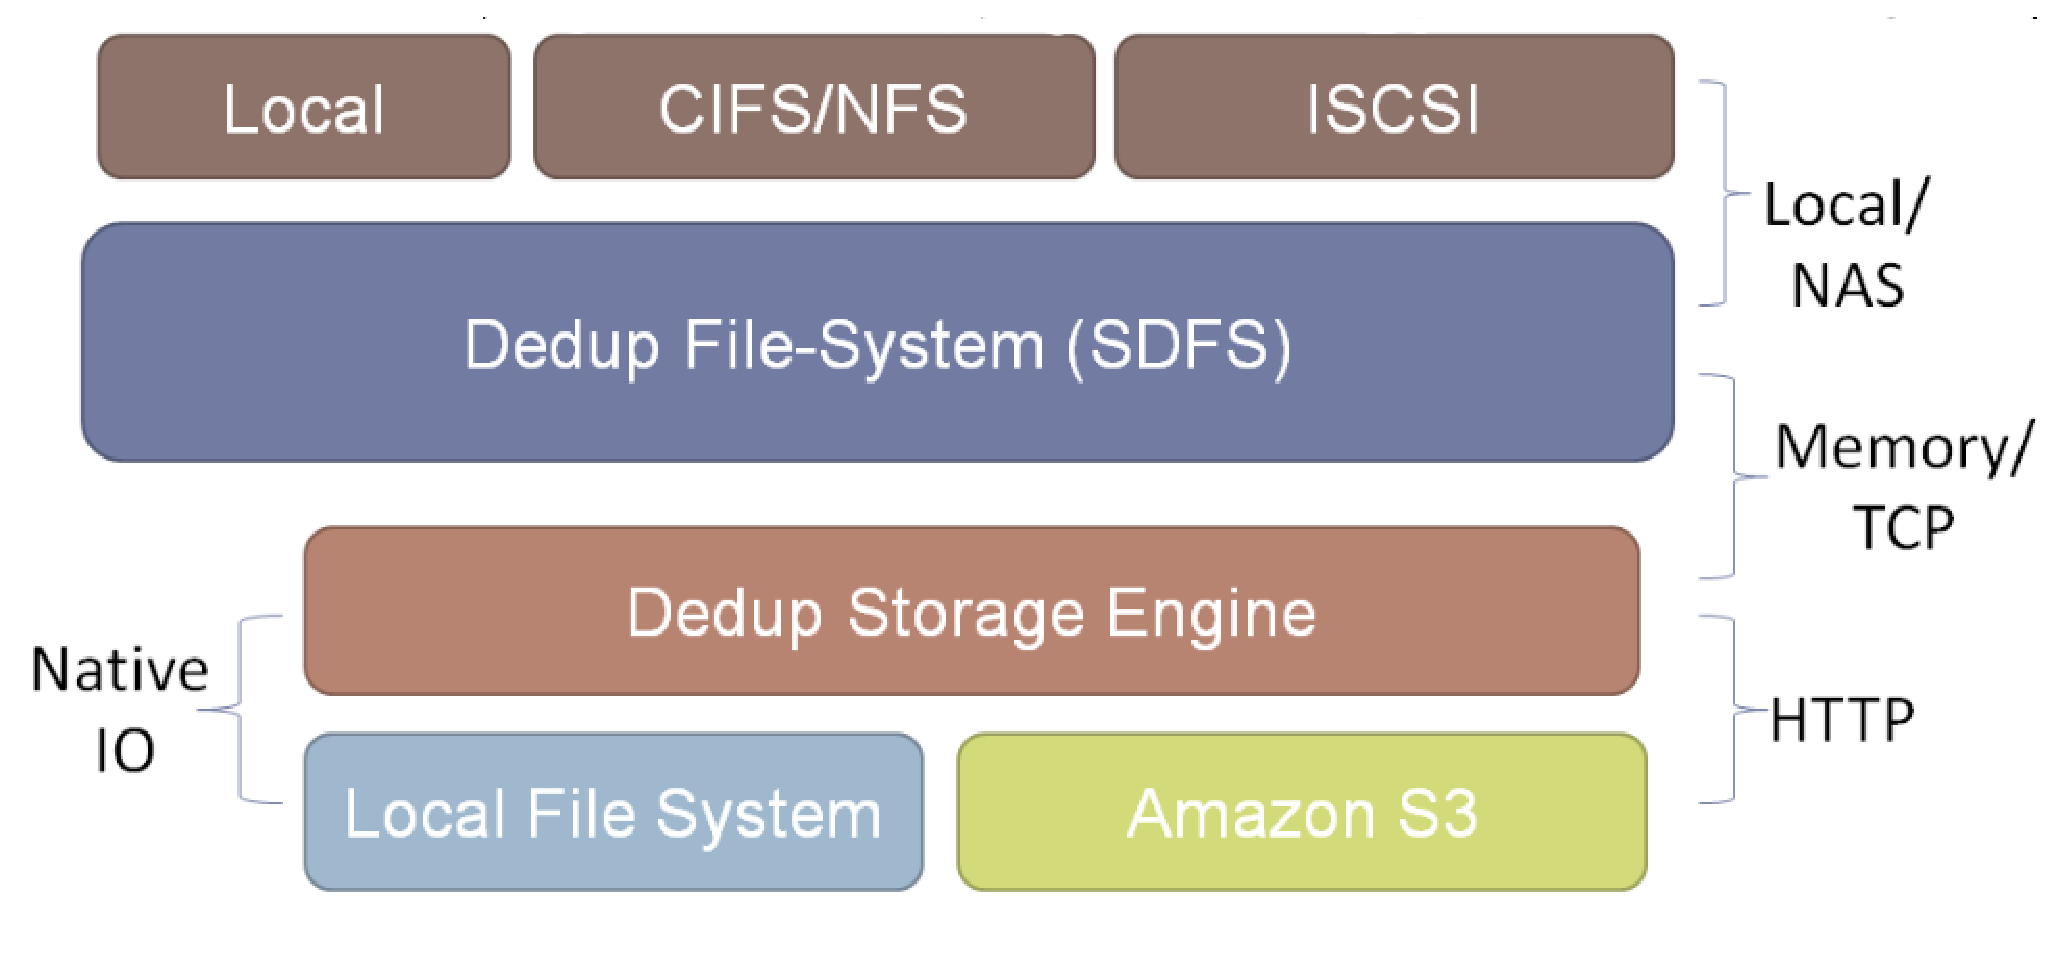
\includegraphics[scale=0.30]{sdfs_arch.eps}
\caption{SDFS Architecture\cite{web:opendedup}}
\end{center}
\end{figure}

\paragraph{}
Figure \ref{fig:sdfsarch} shows that SDFS has a server client design model. The client can be a process on the host machine or a network socket that
writes data to the disk. SDFS integrates with NFS and VFS to support network and local operations. 

